\section{Частично упорядоченные множества. Минимальные элементы, линейно упорядоченные 
множества.  Диаграмма Хассе. Построить диаграмму Хассе указанного множества.}

\begin{definition}
    Множество $M$ с заданным на нем отношением частичного
    порядка называется \textit{частично упорядоченным}.
    (для записи частично упоряденных множеств часто употребляют $\leq$)
\end{definition}

Пусть в множестве $M$ задана частичная упорядоченность. Элементы $a$ и
$b$ называются \textit{сравнимыми}, если $a \leq b$ или $b \leq a$. Далеко не всегда два
элемента из $M$ обязаны быть сравнимыми -- именно по этой причине говорят
о "частичной упорядоченности".

\begin{definition}
    \textit{Минимальным элементом частично упорядоченного
    множества} называется элемент, для которого не существует элемента,
    меньшего его.
    Минимальных элементов может быть несколько.
\end{definition}

\begin{definition}
    Частично упорядоченное множество, в котором любые
    два элемента сравнимы, называется \textit{линейно упорядоченным множеством} или
    \textit{цепью}.
\end{definition}

\begin{definition}
    \textit{Диаграмма Хассе} -- граф частично упорядоченного множества.
    Не совпадает с графом отношения (нет некоторых ребер).
\end{definition}

Однако не любой ориентированный граф является представлением
частично упорядоченного множества.

Чтобы ориентированный граф представлял частично упорядоченное
множество, необходимо и достаточно чтобы в нем не было циклов. В
математической литературе частично упорядоченные множества часто
изображаются в виде неориентированных графов, при этом подразумевается,
что предшествующие элементы расположены ниже последующих. Поэтому,
если в этих схемах правильно заменить ребра на ориентированные, то все они
окажутся направленными снизу вверх (иногда наоборот сверху вниз).

\newpage
Пример диаграммы Хассе для множества $R = \set{3, 4, 12, 24, 48, 72 | \vdots}$

Отношение состоит из следующих пар.
R={(3,12), (3,24), (3,48), (3,72), (4,12), (4,24), (4,48), (4,72), (12,24), (12,48), (12,72), (24,48), (24,72), (3,3), (4,4), (12,12), (24,24), (48,48), (72,72)} \\
Диаграмма Хассе будет иметь вид:

\begin{figure}[h]
    \centering
    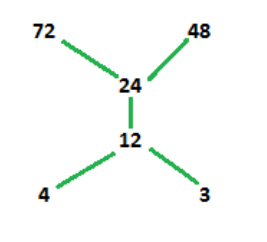
\includegraphics[scale=0.5]{11.png}
\end{figure}

На приведенной выше диаграмме элементы 3 и 4 находятся на одном уровне,
поскольку они не связаны друг с другом и меньше других элементов в
наборе. Следующий последующий элемент для 3 и 4 — это 12, т. е. 12 делится и
на 3, и на 4. Тогда 24 делится на 3, 4 и 12. Следовательно, оно помещается выше
12. 24 делит и 48, и 72, но 48 — не делит 72. Следовательно, 48 и 72 не
соединяются.

На нашей диаграмме мы можем видеть транзитивность по мере увеличения
уровня.